\begin{appendices}
\subsection{Code for the Lane Detection algorithm}\label{laneDetect}
\begin{python}
import cv2
import numpy as np
 
def make_points(image, line):
    slope, intercept = line
    y1 = int(image.shape[0])# bottom of the image
    y2 = int(y1*3/5)         # slightly lower than the middle
    x1 = int((y1 - intercept)/slope)
    x2 = int((y2 - intercept)/slope)
    return [[x1, y1, x2, y2]]
 
def average_slope_intercept(image, lines):
    left_fit    = []
    right_fit   = []
    if lines is None:
        return None
    for line in lines:
        for x1, y1, x2, y2 in line:
            fit = np.polyfit((x1,x2), (y1,y2), 1)
            slope = fit[0]
            intercept = fit[1]
            if slope < 0: # y is reversed in image
                left_fit.append((slope, intercept))
            else:
                right_fit.append((slope, intercept))
    # add more weight to longer lines

    if len(left_fit) and len(right_fit):
    #over-simplified if statement (should give you an idea of why the error occurs)
       left_fit_average  = np.average(left_fit, axis=0)
       right_fit_average = np.average(right_fit, axis=0)
       left_line  = make_points(image, left_fit_average)
       right_line = make_points(image, right_fit_average)
       averaged_lines = [left_line, right_line]
       return averaged_lines
 
def canny(img):
    gray = cv2.cvtColor(img, cv2.COLOR_RGB2GRAY)
    kernel = 5
    blur = cv2.GaussianBlur(gray,(kernel, kernel),0)
    canny = cv2.Canny(gray, 50, 150)
    return canny
 
def display_lines(img,lines):
    line_image = np.zeros_like(img)
    if lines is not None:
        for line in lines:
            for x1, y1, x2, y2 in line:
                cv2.line(line_image,(x1,y1),(x2,y2),(0,255,0),10)
    return line_image
 
def region_of_interest(canny):
    height = canny.shape[0]
    width = canny.shape[1]
    mask = np.zeros_like(canny)
 
    triangle = np.array([[
    (200, height),
    (550, 250),
    (1100, height),]], np.int32)
 
    cv2.fillPoly(mask, triangle, 255)
    masked_image = cv2.bitwise_and(canny, mask)
    return masked_image
 

# Code for the detection in an image named 'test_image.jpg'
image = cv2.imread('test_image.jpg')
lane_image = np.copy(image)
lane_canny = canny(lane_image)
cropped_canny = region_of_interest(lane_canny)
lines = cv2.HoughLinesP(cropped_canny, 2, np.pi/180, 100, np.array([]), minLineLength=40,maxLineGap=5)
averaged_lines = average_slope_intercept(image, lines)
line_image = display_lines(lane_image, averaged_lines)
combo_image = cv2.addWeighted(lane_image, 1, line_image, 1, 1)
cv2.imshow("result", combo_image)
cv2.waitKey(0)
cv2.destroyAllWindows()

# Code for the detection in a video named 'test2.mp4'
#cap = cv2.VideoCapture("test2.mp4")
#while(cap.isOpened()):
#    _, frame = cap.read()
#    canny_image = canny(frame)
#    cropped_canny = region_of_interest(canny_image)
#    lines = cv2.HoughLinesP(cropped_canny, 2, np.pi/180, 100, np.array([]), minLineLength=40,maxLineGap=5)
#    averaged_lines = average_slope_intercept(frame, lines)
#    line_image = display_lines(frame, averaged_lines)
#    combo_image = cv2.addWeighted(frame, 0.8, line_image, 1, 1)
#    cv2.imshow("result", combo_image)
#    if cv2.waitKey(1) & 0xFF == ord('q'):
#        break
#cap.release()
#cv2.destroyAllWindows()
\end{python}
\clearpage

\subsection{Image at each step in the lane detect algorithm}
\label{imagelaneDetect}
\begin{figure}[!h]
\begin{minipage}{7cm}
\centering
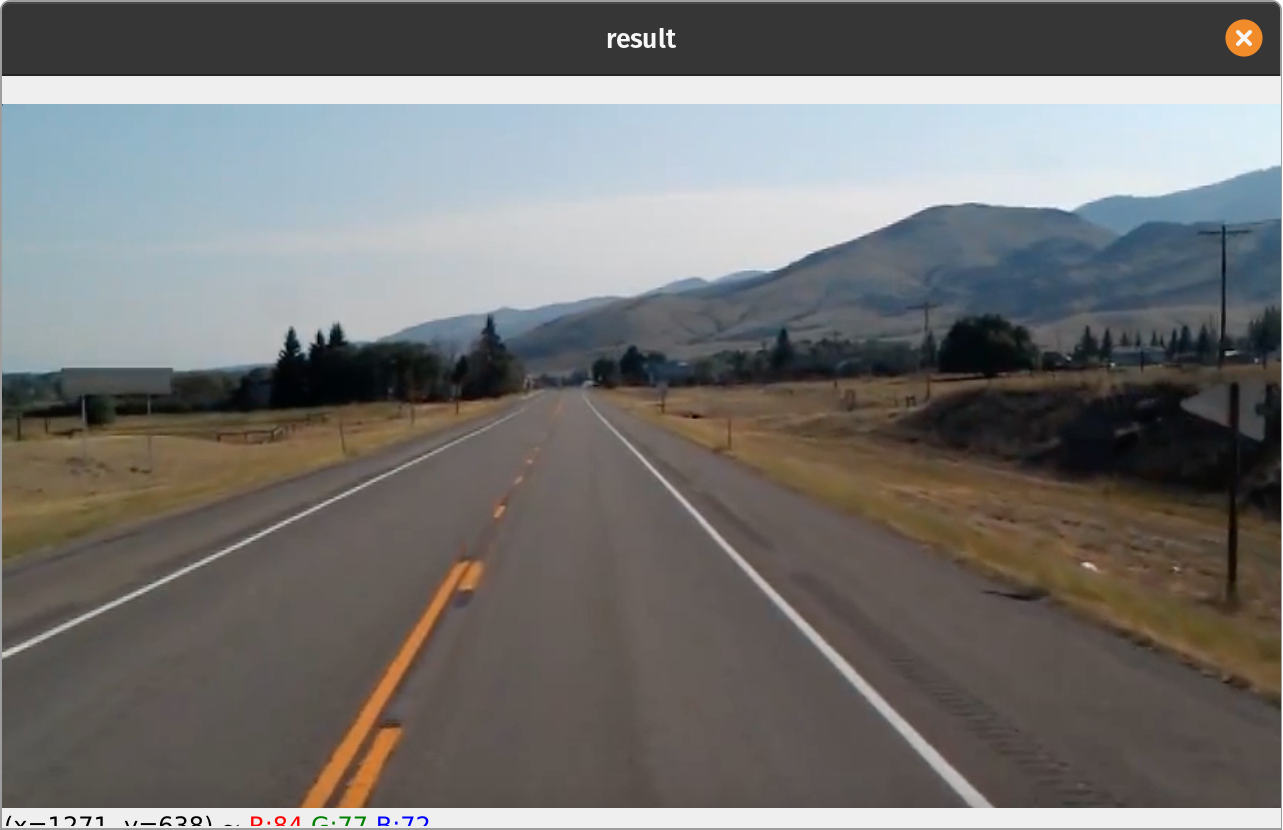
\includegraphics[width=6cm]{img/lane_detect/lane_img.png}
\caption{Original Image}
\end{minipage}
\hspace*{1cm}
\begin{minipage}{7cm}
\centering
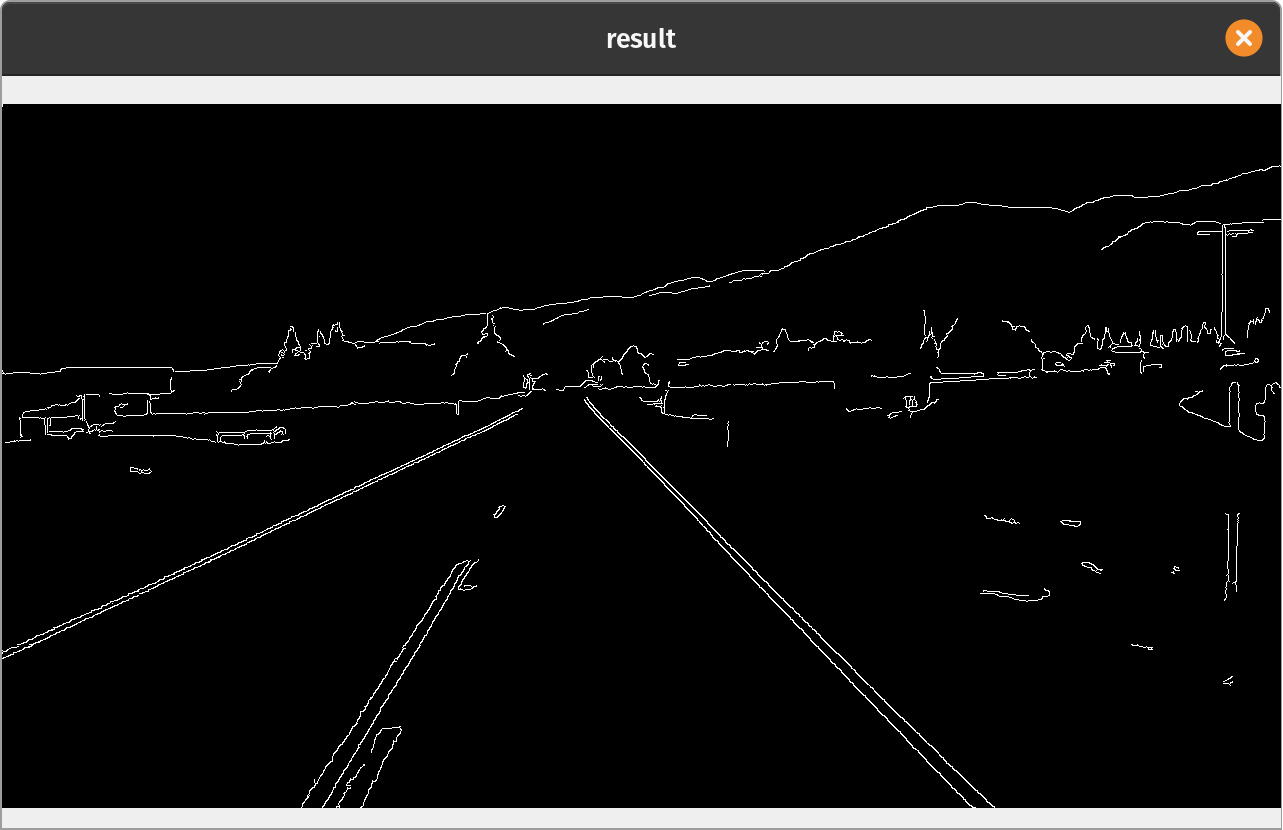
\includegraphics[width=6cm]{img/lane_detect/canny_img.png}
\caption{Gray Image after applying blur and canny-edge detection}
\end{minipage}
\end{figure}

\begin{figure}[!h]
\begin{minipage}{7cm}
\centering
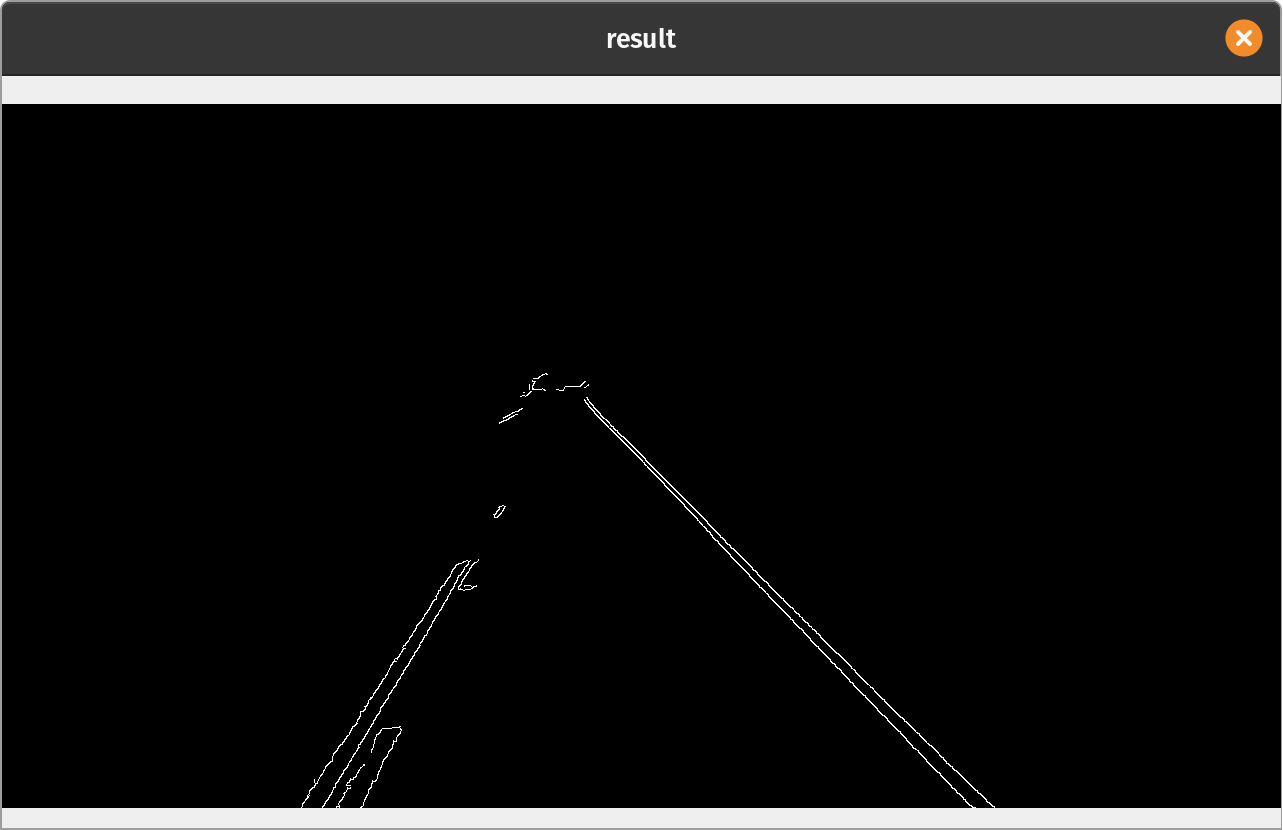
\includegraphics[width=6cm]{img/lane_detect/cropped_img.png}
\caption{We cropped the image to the center triangle}
\end{minipage}
\hspace*{1cm}
\begin{minipage}{7cm}
\centering
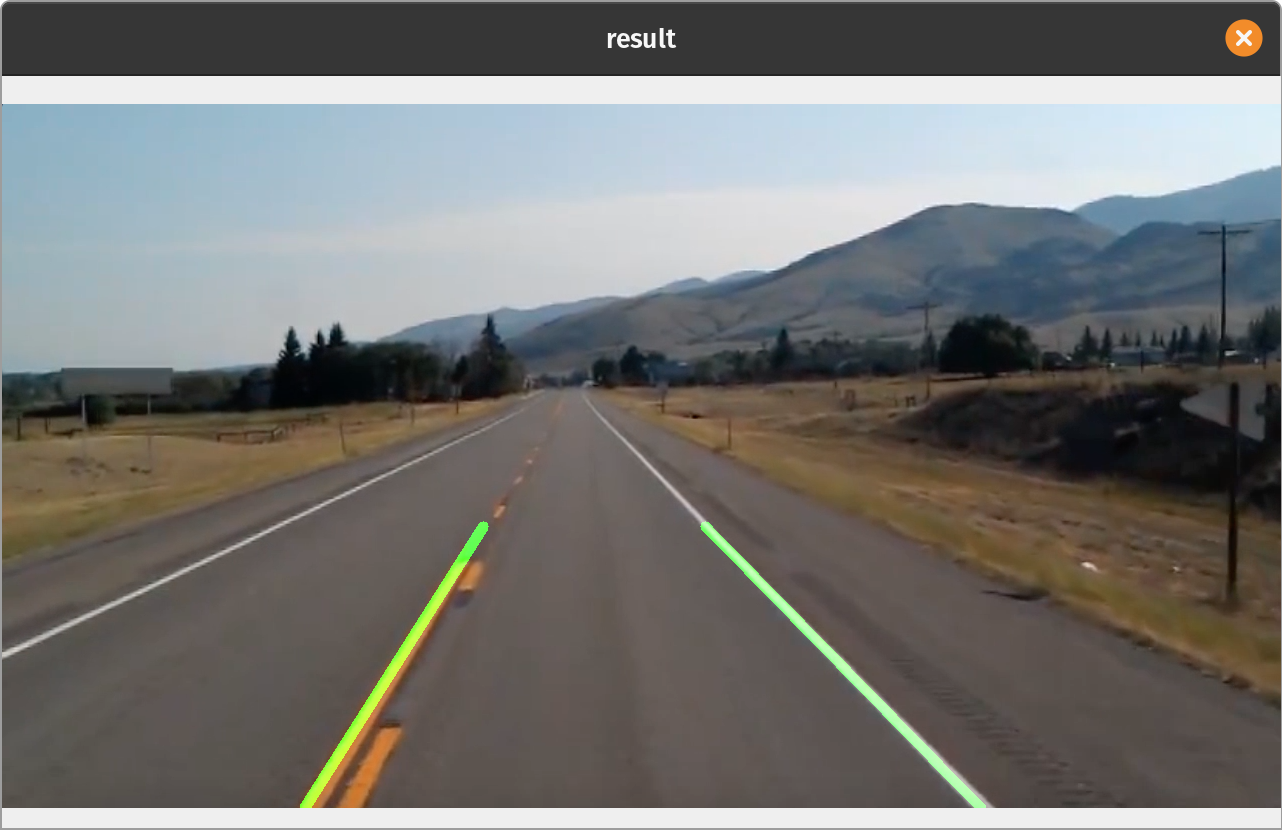
\includegraphics[width=6cm]{img/lane_detect/combo_img.png}
\caption{Final image with superposed detected lines (in green)}
\end{minipage}
\end{figure}

\clearpage
\subsection{TCP Client in Python}
\label{TCPClient}
\begin{python}
import socket
import base64
import requests
import socketio
import sys
import time
import json


# specify Host and Port
HOST = 'localhost'
PORT = 9091


def send_data(steering, throttle, brake):
    msg = str('{"msg_type": "control", "steering": "' +
              str(steering) + '","throttle": "' + str(throttle) +
              '","brake": "' + str(brake) + '"}').encode('utf-8')
    soc.sendall(msg)


def recv_full():
    """
    Test if the msg_type is telemetry, if yes, return the data
    """
    for _ in range(2):
        data = json.loads(soc.recv(8192).decode('utf-8'))
        if not data:
            break
        if data['msg_type'] == 'car_loaded':
            continue
        return json.loads(soc.recv(5000).decode('utf-8'))


def write_data():
    data = recv_full()
    with open('image.jpg', 'wb') as image:
        image.write(base64.b64decode(data['image']))
    with open("data.json", 'w') as f:
        json.dump(data, f)



with socket.socket(socket.AF_INET, socket.SOCK_STREAM) as soc:
    soc.connect((HOST, PORT))
    write_data()



sio = socketio.Client()
\end{python}

\subsection{Financial Management Report}
Next, you can find the financial management report we had to do, inside you will find an overview of the project and the differents approach we took for the budget repartition and the choice of the components of the car.
\includepdf[pages=-]{pdf/PA_finance.pdf}

\end{appendices}